\begin{figure}[ht]
	\begin{subfigure}[b]{0.32\linewidth}
		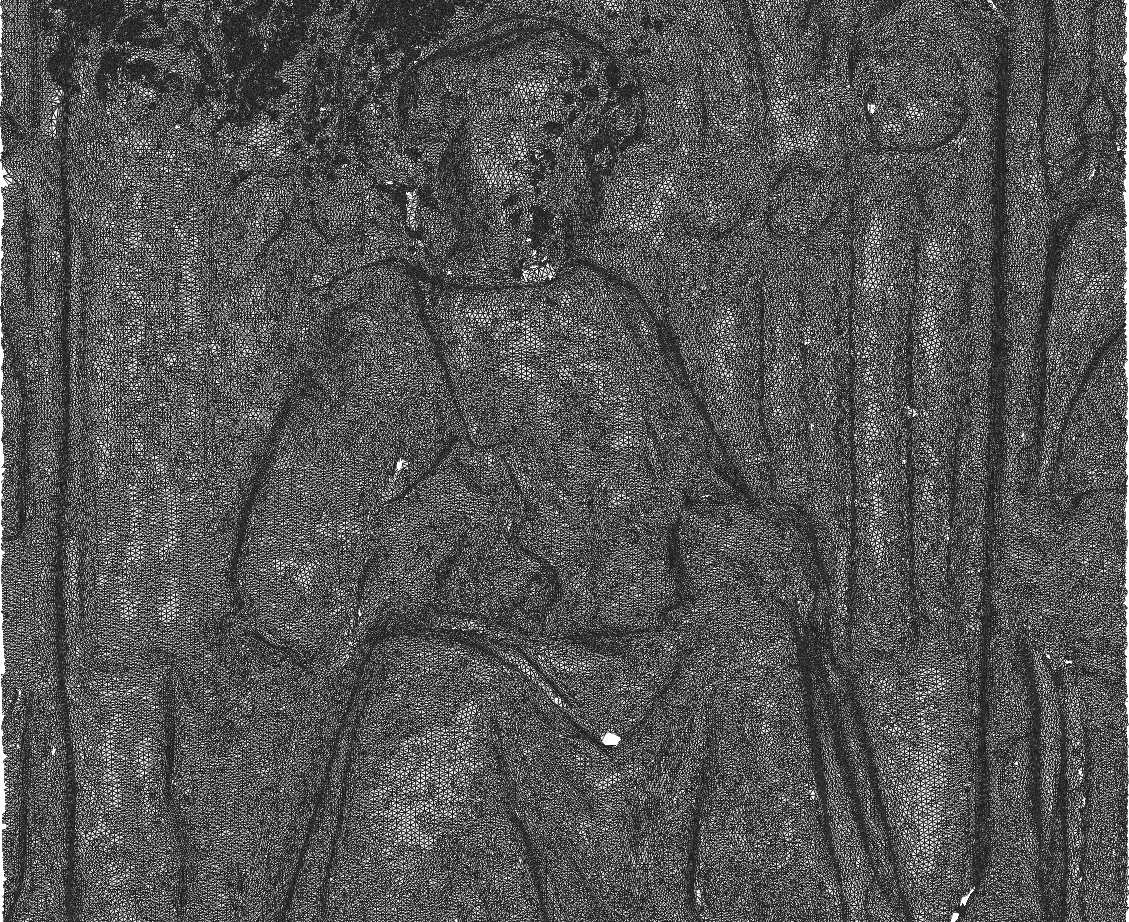
\includegraphics[width=\linewidth]{data/acquired_meshes/unisiegel_wireframe.png}
		\caption{wireframe}\label{fig:unisiegel.a}
	\end{subfigure}
	\begin{subfigure}[b]{0.32\linewidth}
		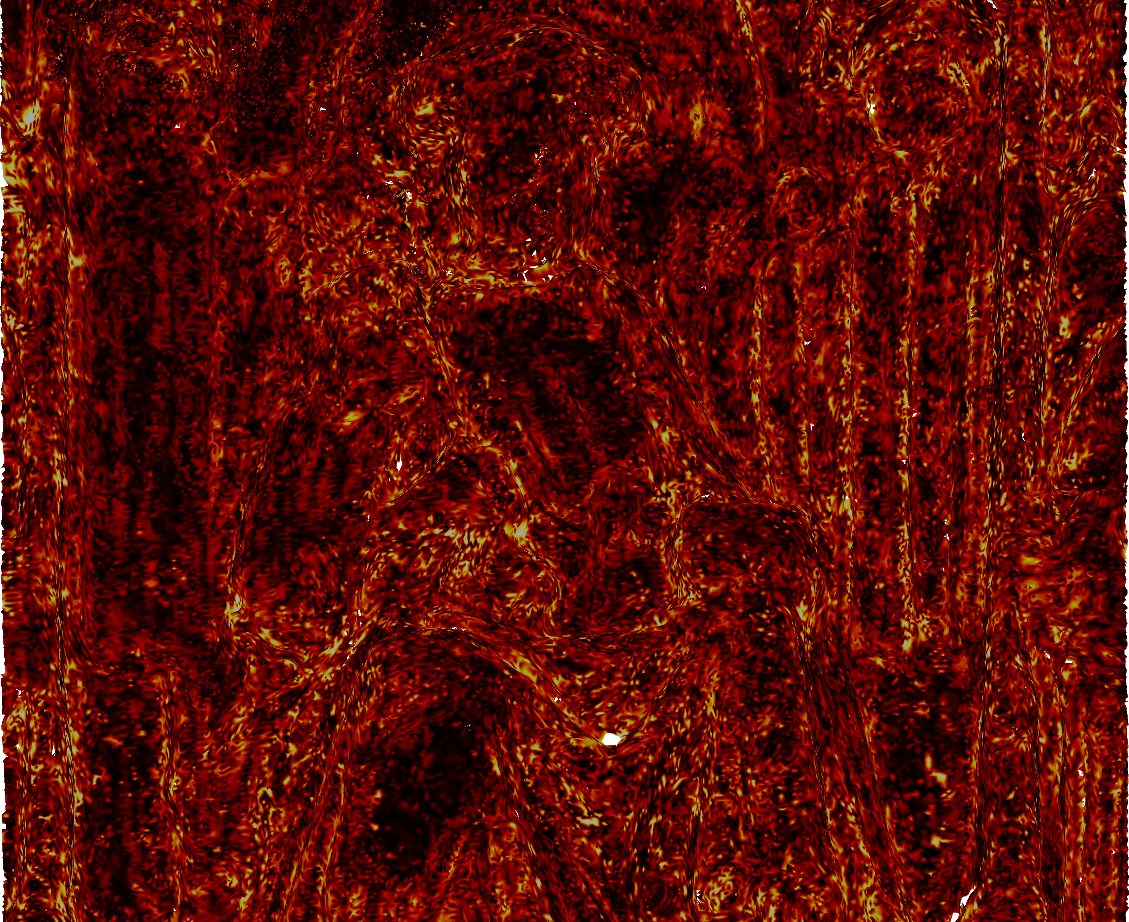
\includegraphics[width=\linewidth]{data/acquired_meshes/unisiegel_0iter.png}
		\caption{$c=0$}\label{fig:unisiegel.b}
	\end{subfigure}
	\begin{subfigure}[b]{0.32\linewidth}
		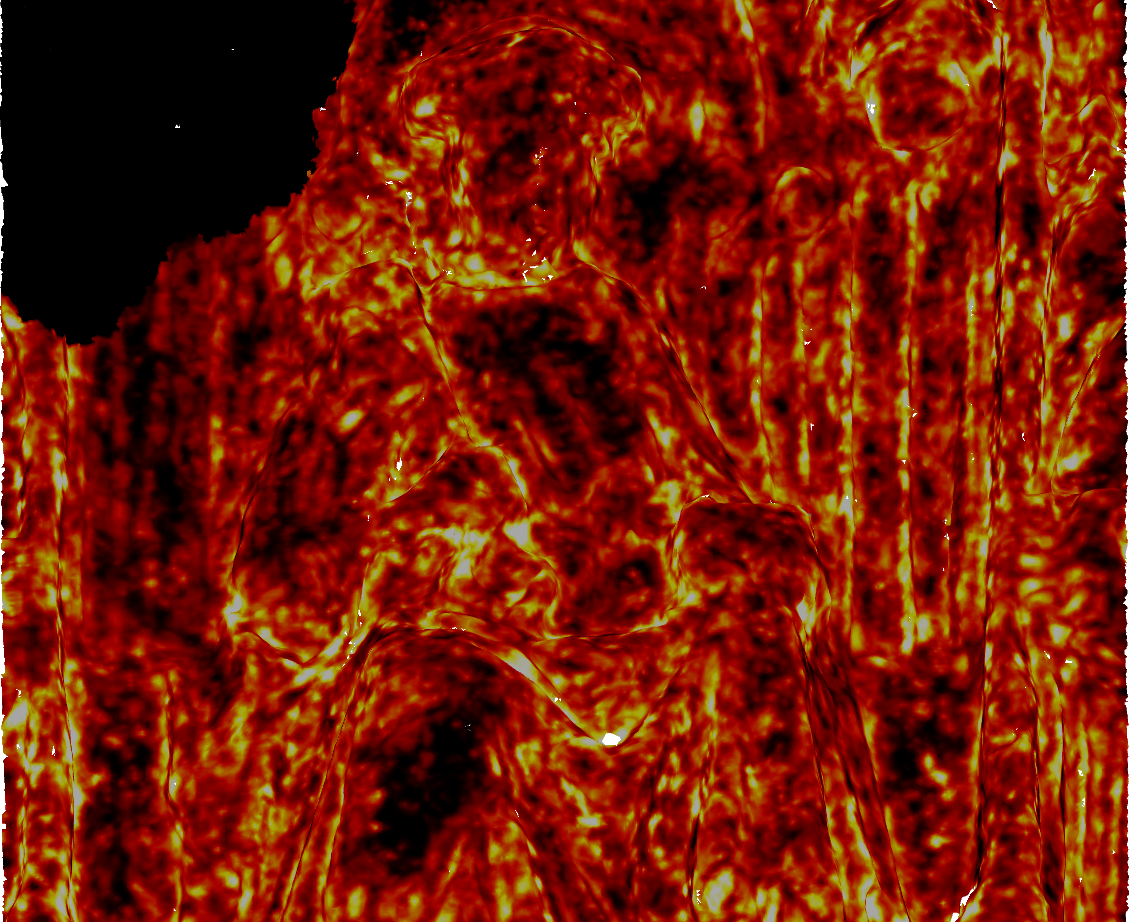
\includegraphics[width=\linewidth]{data/acquired_meshes/unisiegel_100iter.png}
		\caption{$c=100$}\label{fig:unisiegel.c}
	\end{subfigure}
	\caption[Three views of the Univeristy of Heidelberg seal]{Three views of the Univeristy of Heidelberg seal (a) in wireframe (b) colored by MSII function value before convolving the filter (c) colored by function value after convolving the filter 100 times.}
	\label{fig:unisiegel}
\end{figure}
\todoCitation{}
